%%%%%%%%%%%%%%%%%%%%%%%%%%%%%%%%%%%%%%%%%%%%%%%%%%%%%%%%%%%%%%%%%%%%%
% LaTeX Template: Project Titlepage Modified (v 0.1) by rcx
%
% Original Source: http://www.howtotex.com
% Date: February 2014
% 
% This is a title page template which be used for articles & reports.
% 
% This is the modified version of the original Latex template from
% aforementioned website.
% 
%%%%%%%%%%%%%%%%%%%%%%%%%%%%%%%%%%%%%%%%%%%%%%%%%%%%%%%%%%%%%%%%%%%%%%

\documentclass[12pt]{report}
\usepackage[a4paper]{geometry}
\usepackage[myheadings]{fullpage}
\usepackage{fancyhdr}
\usepackage{parskip}
\usepackage{lastpage}
\usepackage{graphicx, wrapfig, subcaption, setspace, booktabs}
\usepackage[T1]{fontenc}
\usepackage[font=small, labelfont=bf]{caption}
\usepackage{fourier}
\usepackage[protrusion=true, expansion=true]{microtype}
\usepackage[english]{babel}
\usepackage{sectsty}
\usepackage{url, lipsum}
\usepackage{indentfirst}
\usepackage{titlesec}
\usepackage{lipsum}
\usepackage{titlesec}
\usepackage{lipsum}
\usepackage{verbatim}
\usepackage{hyperref}
\usepackage{lstcustom}
\usepackage{mathtools}

\titleformat{\chapter}[display]
{\bfseries\Large}                                            
{\filright}
{1ex}{}[]
\setlength{\parindent}{10mm}
\newcommand{\HRule}[1]{\rule{\linewidth}{#1}}
\onehalfspacing
\setcounter{tocdepth}{5}
\setcounter{secnumdepth}{5}
\titleformat{\chapter}[display]
    {\normalfont\huge\bfseries}{\chaptertitlename\ \thechapter}{0pt}{\Huge}
\titlespacing*{\chapter}{0pt}{0pt}{0pt}

\vspace{0pt}

%-------------------------------------------------------------------------------
% HEADER & FOOTER
%-------------------------------------------------------------------------------
\pagestyle{fancy}
\fancyhf{}
\setlength\headheight{3pt}
\fancyhead[L]{}
\fancyhead[R]{\rightmark}
\fancyfoot[R]{\thepage\ . page}
%-------------------------------------------------------------------------------
% TITLE PAGE
%-------------------------------------------------------------------------------

\begin{document}

\title{ \normalsize \textsc{}
		\\ [1.0cm]
		\HRule{0.5pt} \\
		\LARGE \textbf{\uppercase{Neural Networks and Deep Learning}}
		\HRule{2pt} \\ [0.5cm]
		\normalsize \today \vspace*{5\baselineskip}}

\date{}
\author{
		Kerman Sanjuan Malaxechevarria \\
      }




\maketitle
\renewcommand{\contentsname}{Index}
\tableofcontents
\

%-------------------------------------------------------------------------------
% subsection title formatting
\sectionfont{\scshape}
%-------------------------------------------------------------------------------

%-------------------------------------------------------------------------------
% BODY
%-------------------------------------------------------------------------------

\chapter{Introduction to Neural Networks}
\section{Definition and uses}
A neural network is a network or circuit of neurons, composed by artificial neurons. These networks are used on the field of artificial intelligence, specifically, as a machine learning algorithm. The applications of this algorithm are many, for example, hand-writing recognition, this will be the main example of the first chapter.  
As we said , neural networks are circuits made out of neurons. But, what does a neuron mean?  Formally, an artificial neuron is a mathematical function conceived as a model of biological neurons. Each neuron has it's multiple own inputs and a single output, the output will always depend on the inputs and the "type" of neuron. Now, we will talk about Perceptrons, which are the most simple type of artificial neuron.
\begin{figure}[h]
  \caption{Graphical Example of a Neural Network}
  \centering
      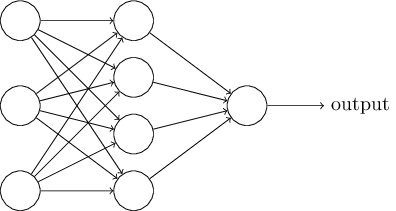
\includegraphics[scale=0.5]{Resources/single-neural-network.png}
\end{figure}
\newpage
\section{Perceptrons}
The perceptron takes a several binary inputs and produces a single binary output. $x_1,x_2,x_3$ are the inputs, and $w_1,w_2,w_3$ the weights , these weights determines the relevance of the input on the output.
\begin{figure}[h]
  \caption{Perceptron}
  \centering
      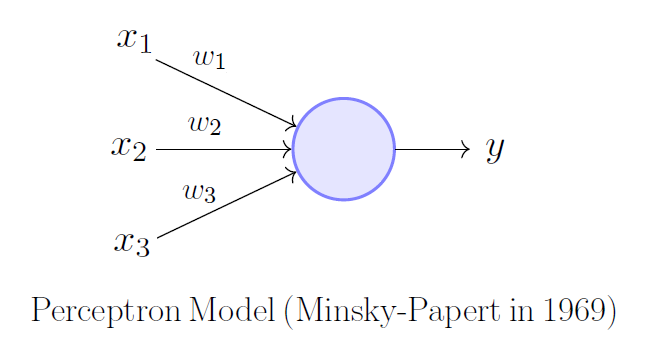
\includegraphics[scale=0.25]{Resources/0_LJBO8UbtzK_SKMog.png}
\end{figure}
In other words, a way you can think about a perceptron is that it's a device that makes decisions by weighing up evidence. 
Depending on the weights and the threshold, we can get different models of decision making.
\begin{equation}
	Desired Output = \begin{cases} 0  & \mbox{if  } \sum{w_j x_j} \leq \mbox{ threshold} \\ 
		1  & \mbox{if  } \sum{w_j x_j} \geq \mbox{ threshold}  \end{cases}
		\end{equation}
Obviously, with only one perceptron we are not able to create a neural network, thats because they're structured in such a way that three layers are generated (in most of cases). 
\begin{figure}[h]
  \caption{Basic Structure of a Neural Network}
  \centering
      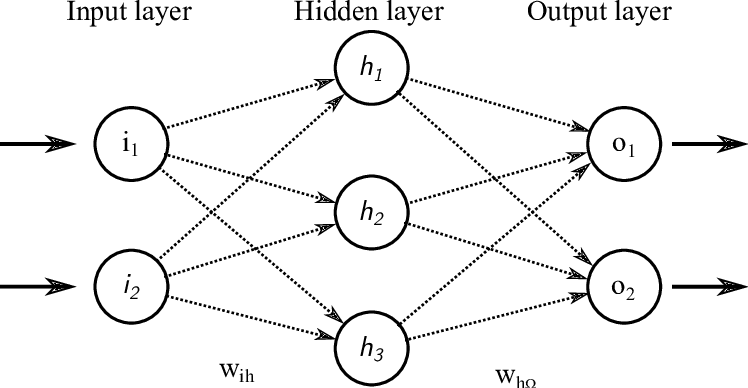
\includegraphics[scale=0.25]{Resources/Example-for-an-artificial-neural-network-with-two-input-neurons-two-hidden-neurons-and.png}
\end{figure}

The first layer of perceptrons, also named as input layer, makes simple decisions, wheighing inputs and making simple decisions. Furthermore, the second layer, also called hidden layer, will make more complex decisions. This process will repeat until the last layer, the output one, where the decision will be displayed. 
\newpage

	The before mentioned $\sum{w_j x_j} \leq \mbox{ threshold}$ equation is a bit complicated and no intuitive, another way to explain the same is changing $ b \equiv -threshold$ . The bias can be explained as how easy gets it is to get a 1 as output. For a perceptron with really big bias , it's easy to output a one, instead, with a very large negative number, it will be hard. 
	It's important to mention that, if the Perceptron has two inputs, and both have the same weight, the perceptron will work as NAND gate, taking this into account, we can make every logic gate using perceptrons. 
 

\section{Sigmoid Neurons}
Sigmoid Neurons are one of the most relevant types of neurons, unlike perceptrons, a little change  the weights will just make a little corresponding change on the output. This fact makes sigmoid neurons perfect for learning, because we can adjust the weights according to the desired output. In other words, we could modify the weights and the biases to get the network to behave more in the manner we want. This isn't happens when our network contains perceptrons, in fact, a small change on the inputs will make sometimes to flip completely the output. 

The mathematical difference between perceptrons and sigmoid neurons, is the due to the  fact that they have different equations. In the case of the sigmoid, the following equation defines the output.
\begin{figure}[h]
  \caption{Sigmoid Equation}
  \centering
      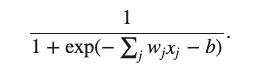
\includegraphics[scale=0.5]{Resources/SigmoidEquation}
\end{figure}
	
	Maybe this isn't the best way to see the difference, so lets see the plot of both neuron types
	\begin{figure}[h]
  \caption{Sigmoid Equation Plot}
  \centering
      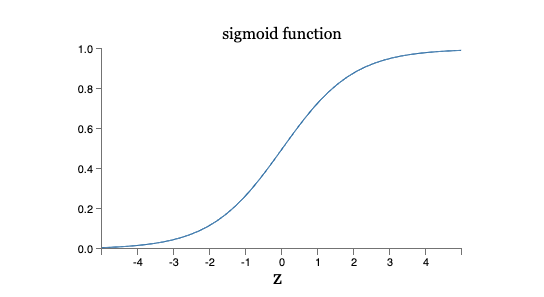
\includegraphics[scale=0.5]{Resources/SigmoidPlot}
\end{figure}




And now, the plot of the perceptron.





\begin{figure}[h]
  \caption{Perceptron Equation Plot}
  \centering
      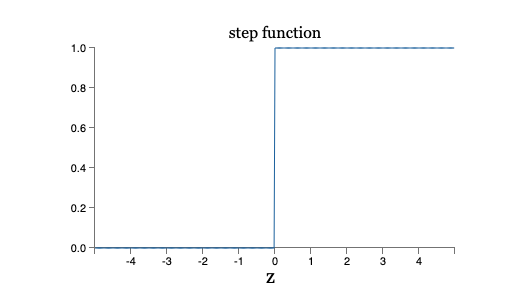
\includegraphics[scale=0.5]{Resources/PerceptronPlot}
\end{figure}
	
	
	    
	    
	   aaa
	As we see, the reason of  the difference of outputs is clear, sigmoid makes a slower change, instead of perceptron which makes a big step.
\end{document}


%-------------------------------------------------------------------------------
% SNIPPETS
%-------------------------------------------------------------------------------

%\begin{figure}[!ht]
%	\centering
%	\includegraphics[width=0.8\textwidth]{file_name}
%	\caption{}
%	\centering
%	\label{label:file_name}
%\end{figure}

%\begin{figure}[!ht]
%	\centering
%	\includegraphics[width=0.8\textwidth]{graph}
%	\caption{Blood pressure ranges and associated level of hypertension (American Heart Association, 2013).}
%	\centering
%	\label{label:graph}
%\end{figure}

%\begin{wrapfigure}{r}{0.30\textwidth}
%	\vspace{-40pt}
%	\begin{center}
%		\includegraphics[width=0.29\textwidth]{file_name}
%	\end{center}
%	\vspace{-20pt}
%	\caption{}
%	\label{label:file_name}
%\end{wrapfigure}

%\begin{wrapfigure}{r}{0.45\textwidth}
%	\begin{center}
%		\includegraphics[width=0.29\textwidth]{manometer}
%	\end{center}
%	\caption{Aneroid sphygmomanometer with stethoscope (Medicalexpo, 2012).}
%	\label{label:manometer}
%\end{wrapfigure}

%\begin{table}[!ht]\footnotesize
%	\centering
%	\begin{tabular}{cccccc}
%	\toprule
%	\multicolumn{2}{c} {Pearson's correlation test} & \multicolumn{4}{c} {Independent t-test} \\
%	\midrule	
%	\multicolumn{2}{c} {Gender} & \multicolumn{2}{c} {Activity level} & \multicolumn{2}{c} {Gender} \\
%	\midrule
%	Males & Females & 1st level & 6th level & Males & Females \\
%	\midrule
%	\multicolumn{2}{c} {BMI vs. SP} & \multicolumn{2}{c} {Systolic pressure} & \multicolumn{2}{c} {Systolic Pressure} \\
%	\multicolumn{2}{c} {BMI vs. DP} & \multicolumn{2}{c} {Diastolic pressure} & \multicolumn{2}{c} {Diastolic pressure} \\
%	\multicolumn{2}{c} {BMI vs. MAP} & \multicolumn{2}{c} {MAP} & \multicolumn{2}{c} {MAP} \\
%	\multicolumn{2}{c} {W:H ratio vs. SP} & \multicolumn{2}{c} {BMI} & \multicolumn{2}{c} {BMI} \\
%	\multicolumn{2}{c} {W:H ratio vs. DP} & \multicolumn{2}{c} {W:H ratio} & \multicolumn{2}{c} {W:H ratio} \\
%	\multicolumn{2}{c} {W:H ratio vs. MAP} & \multicolumn{2}{c} {\% Body fat} & \multicolumn{2}{c} {\% Body fat} \\
%	\multicolumn{2}{c} {} & \multicolumn{2}{c} {Height} & \multicolumn{2}{c} {Height} \\
%	\multicolumn{2}{c} {} & \multicolumn{2}{c} {Weight} & \multicolumn{2}{c} {Weight} \\
%	\multicolumn{2}{c} {} & \multicolumn{2}{c} {Heart rate} & \multicolumn{2}{c} {Heart rate} \\
%	\bottomrule
%	\end{tabular}
%	\caption{Parameters that were analysed and related statistical test performed for current study. BMI - body mass index; SP - systolic pressure; DP - diastolic pressure; MAP - mean arterial pressure; W:H ratio - waist to hip ratio.}
%	\label{label:tests}
%\end{table}